\documentclass[11pt]{article}
\usepackage{colacl}
\usepackage{graphicx}
\usepackage[utf8]{inputenc}
\usepackage[dvipsnames]{xcolor}
\usepackage[inline]{enumitem}
\sloppy

%used for identifying drafting or notes
\newcommand{\drafting}[1]{\textcolor{OliveGreen}{#1}}

\title{COMP30027 Assignment 2 Report}
\author
{Anonymous}

\renewcommand\labelenumi{(\theenumi)}

\begin{document}
\maketitle

\section{Introduction}
The goal of this project was to predict the star ratings of a review of a restaurant based on the review text. The data available for learning and evaluation consisted of approximately 250000 Yelp reviews, and is made available by \cite{medhat_sentiment_2014} and \cite{rayana_collective_2015}. Each review consists of the review text, a rating (1, 3 or 5 stars) and review metadata (which was not used). We sought to investigate to what extent it was possible to predict the rating of a review from the review text alone. 

\section{Background}
This task is a type of sentiment analysis: the task of predicting sentiment from text. Performing sentiment analysis first requires extracting features from text via some encoding. One common method is to convert a text to a Bag-of-words (BOW), in which entries consist of word frequencies. This is method is simple, although has the disadvantage of producing very high dimensional features and not representing word ordering \cite{le_distributed_2014}. A more sophisticated technique is Paragraph Vector Encoding (PVE), which uses a neural network to embed texts within an abstract vector space in such a way that semantically similar texts are closer \cite{le_distributed_2014}.

Sentiment analysis tasks tend to deal with high dimension, sparse, and correlated features. This often leads to classes being linearly separable, making support vector machine models a popular choice \cite{medhat_sentiment_2014}. In terms of probabilistic classifiers, logistic regression models tend to perform well on sentiment analysis tasks since they do not assume features are independent, in contrast to other probabilistic classifiers like na\"{i}ve Bayes \cite{medhat_sentiment_2014}.

\section{Method} \label{sec:method}
We investigated models based on logistic regression (detailed in Section \ref{subsec:method-lr}) and support vector machine (detailed in Section \ref{subsec:method-svm}) techniques, in each case using the implementations made available through the Scikit Learn Python library \cite{sklearn_pedregosa_scikit-learn_2011}. These models used paragraph vector encodings of the review text, which was produced using the implementation made available through the Gensim Python library \cite{gensim_rehurek_software_2010}. 

\drafting{Move to results?}
In addition to model-specific hyperparameters (which will be discussed in the respective sections) the dimension of the parameter vector space embedding is a hyperparameter for all of our models. This can be interpreted as a measure of complexity of the model. As the dimension of the paragraph vector encoding a review increases, the degree to which the paragraph vector can capture the information in the review will increase too. Not all of the information in a review is likely to be useful for this classification task however\footnote{Review text also may contain information such as the cuisine of the restaurant, the time-of-day of the visit and the gender of the wait-staff, much of which is likely irrelevant to the task at hand.}, so there is a point at which increasing the dimension of the feature space will lead to over-fitting and degrade the performance of the classifier.
\subsection{Feature Selection} \label{subsec:method-features}

We investigated two text features, Bag-of-words and Paragraph Vector Encoding. We used Principle Component Analysis and Singular Value Decomposition to visualise each feature in 2 dimensions. We found that PVE better separated the instances of each class as distinct clusters were more visible.

When used to train a basic Logistic Regression model, PVE resulted in a much higher accuracy than BOW. We then combined the K-best words by Chi-square score (for an increasing number K) from the BOW as attributes to PVE and observed no significant increase in accuracy.

We decided to use PVE to train all subsequent models.
\subsection{Logistic regression} \label{subsec:method-lr}
\drafting{
We investigated a single Logistic Regression model for multi-class classification; Multinomial Logistic Regression (MLR).
MLR has a single hyperparameter C, which is the inverse of the L2-Regularisation strength, a measure of how strictly the model fits to the training data and avoids mis-classifying training instances.
We investigated two ensembling techniques on MLR, Boosting and Bagging.}
\subsubsection*{Justifying Logistic Regression model selection}
\drafting{
Several techniques exist for multi-class classification using Logistic Regression, such as training multiple binary Logistic Regressors (one for each class label) using a One-versus-rest scheme and predicting based on the model with the highest score, or Ordinal Logistic Regression, which is particularly suited for ordinal class labels.
One-versus-rest models are less efficient, tending to have larger standard errors \cite{zbMATH01817585}.
Ordinal Logistic Regression is not implemented as part of the standard Scikit Learn Python library and thus was not investigated due to time constraints.
}

\drafting{
Thus MLR was chosen as a probabilistic model for comparison with deterministic models such as SVM.
}

\subsection{Support vector machine} \label{subsec:method-svm}
We investigated three variants of support vector machine (SVM) classifiers: a SVM with a linear kernel and one-verses-rest multi-class classification (Linear-SVM), a SVM model with a radial basis function (RBF) kernel and one-verses-rest multi-class classification (RBF-SVM), and a SVM with a linear kernel separating the positive and negative sentiment classes, in which marginal instances are classified as having neutral sentiment (Binary-SVM). 

All three SVM-based model have a regularisation coefficient $C$ as a hyperparameter, which determines the trade-off between margin maximisation and training error minimisation. As $C$ increases the margin is increased, however more training instances are allowed to be misclassified. The RBF-SVM also has the kernel hyperparameter $\gamma$, which in this case was used to scale $\frac{1}{\textrm{Var}(X) \cdot numfeatures}$ (\drafting{explain this better}). The Binary-SVM has the probability threshold hyperparameter, which is the probability a negative of positive sentiment prediction must exceed to be classified as that class \drafting{awkward wording here}.

\subsubsection*{Justifying SVM model selection}
Paragraph vector encoding is well suited to classification by an SVM model since paragraph vectors have meaningful geometric relationships to one another \cite{le_distributed_2014}, and SVM models attempt to exploit the geometry of the feature space by fitting a separating hyperplane. For example, the relative distance between points in the paragraph vector space is relevant to their relative meaning. This is in contrast Bag-of-Words vectors, in which the vector encodings of the (one word) texts ``horrible'', ``terrible'' and ``great'' are equidistant in the Bag-of-Words feature space.

The paragraph vector encoding of text is also designed to transfer relationships in the meaning of text to linear relationships between paragraph vectors: ``king'' - ``man'' + ``woman'' = ``queen'' \cite{le_distributed_2014}. If we suppose that negative and positive sentiment reviews have exactly opposite meanings (with neutral sentiment reviews somewhere in between) then we would expect the review text of these classes to be linearly separable with the paragraph vector encoding. Preliminary testing of different kernel functions (without tuning any hyperparameters) indeed showed that an SVM classifier with a linear kernel performed the best in every metric, however an SVM classifier came quite close in performance. For this reason we chose to continue with extended analysis of both.

Under the assumption that positive and negative sentiment reviews are exactly opposite in meaning and that neutral sentiment reviews are some mixture (i.e. a linear combination in paragraph vector space) of positive and negative meanings, it seems plausible that the neutral sentiment reviews will lie close to the hyperplane which separates the positive and negative sentiment reviews. This encourages the consideration of a binary SVM classifier which distinguishes positive and negative reviews, where instances which fall in the margin are classified as neutral. Rather than using the raw distance to the hyperplane, opted to use a probabilistic variant of SVM which estimates the probability of an instance belonging to each class based on its distance to the hyperplane \cite{platt_probabilistic_1999}. This allowed us to use a probability threshold $p_T$ for neutral classification as a hyperparameter, rather than a distance threshold, which means the value of this threshold is independent of the specific paragraph vector embedding\footnote{The specific embedding of a particular text is only relevant in the context of the training corpus used to compute the embedding function \cite{le_distributed_2014}.}. A probability threshold also has the benefit of making the model more interpretable. Despite its apparent theoretical foundations, results in the literature suggest that such a classifier will always result in worse performance as compared to using a standard multi-class approach \cite{koppel_importance_2006}. Nevertheless we chose to pursue this approach as well.


\subsection{Stacking model}
\drafting{
We investigated Stacking as an ensemble technique to improve the performance of our base classifiers. We stacked all combinations of our best classifiers, Logistic Regression, RBF SVM and Linear SVM, including all three. For every combination, we used the parameters found to be the best for each base classifier alone. This included the PVE dimension. Logistic Regression was used as the meta-classifier in each case (with no parameter tuning).
We further analysed the performance of the best stacked classifier in detail.
}

\section{Results}
\drafting{discussion of why we used stratified splits? We used stratified K-fold cross validation to ensure that the distribution of class labels in the training data was consistent among partitions}
In order to identify the optimal feature space dimension for each model, we first evaluated our model \drafting{(using what metric? evaluated our model accuracy and F1 score on...)} (with hyperparameters untuned) on paragraph vector of dimensions 25 to 300 in steps of 25 encodings using an 80:20 stratified random holdout, only using the training set in each case to compute the paragraph vector embedding function. A random holdout method, rather than cross-validation, was used due to the computation expense of computing paragraph vector encodings: producing cross-validation splits for many dimensions was out of the question. For the RBF-SVM and Binary-SVM models this dimension was 125, and for the Linear-SVM and MLR models this dimension was 150.

\drafting{Why cross validaton? (to prevent overfitting the hyperparameters)}
We then computed the paragraph vector encodings for a 5-fold stratified cross validation split at that dimension, again only using the training set of each split to produce the encoding. This pre-computed split was then used to tune the remaining hyperparameters. Since each cross validation run \drafting{took a long time} parameter values were initially adjusted in large increments, and then a finer full grid search was done on regions of interest. We found that the best hyperparameter values were: for Linear-SVM $C = 0.009$, for RBF-SVM $(C, \gamma) = (1.25, 0.6)$ (Figure \ref{fig:rbf-gridsearch}), for Binary-SVM $(C, p_T) = 0.0025, 0.9)$ (Figure \ref{fig:binary-gridsearch}), and for MLR $C = 0.015$.
\begin{figure}
	\centering
	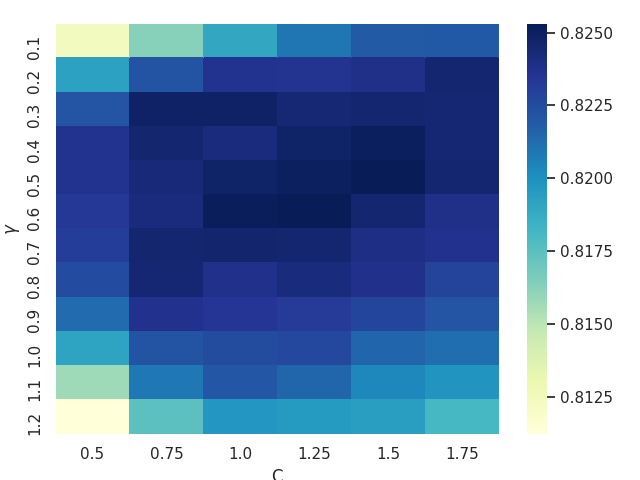
\includegraphics[width = 0.3\textwidth]{fig-rbf-gridsearch.png}
	\caption{RBF-SVM Gridsearch}
	\label{fig:rbf-gridsearch}
\end{figure}

\begin{figure}
	\centering
	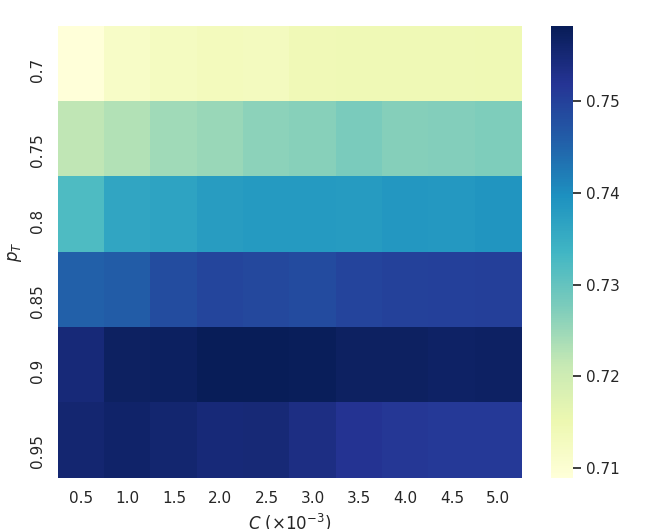
\includegraphics[width = 0.3\textwidth]{fig-binary-gridsearch.png}
	\caption{Binary-SVM Gridsearch}
	\label{fig:binary-gridsearch}
\end{figure}

After tuning the hyperparameters, we evaluated the final model trained on paragraph vectors of dimensions from 25 to 300 in steps of 25 to produce the learning curve in Figure \ref{fig:learning-curve}. 
\begin{figure}
	\centering
	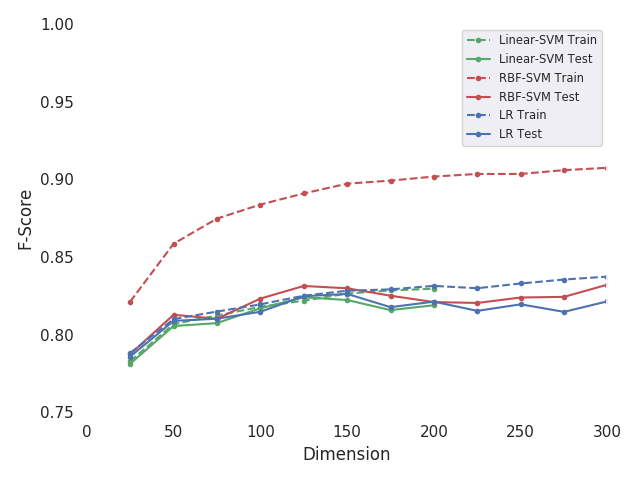
\includegraphics[width = 0.3\textwidth]{learning-curves.png}
	\caption{Learning curve}
	\label{fig:learning-curve}
\end{figure}


As discussed in Section \ref{sec:method} the dimension of the paragraph vector encoding is a measure of the complexity of our model. We also evaluated our model on the 5-fold cross validation split at the optimal dimension, the results of which can be seen in Figures \ref{fig:binary-cm}, \ref{fig:linear-cm}, \ref{fig:rbf-cm}, \ref{fig:lr-cm}. 
\begin{figure}
	\centering
	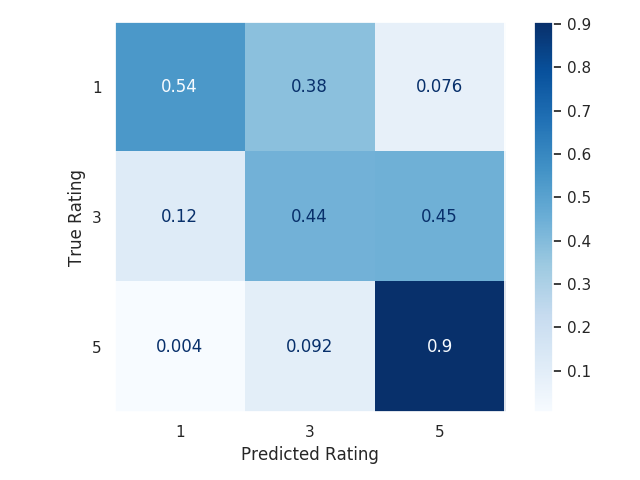
\includegraphics[width = 0.3\textwidth]{fig-binary-cm.png}
	\caption{Binary-SVM Confusion Matrix}
	\label{fig:binary-cm}
\end{figure}

\begin{figure}
	\centering
	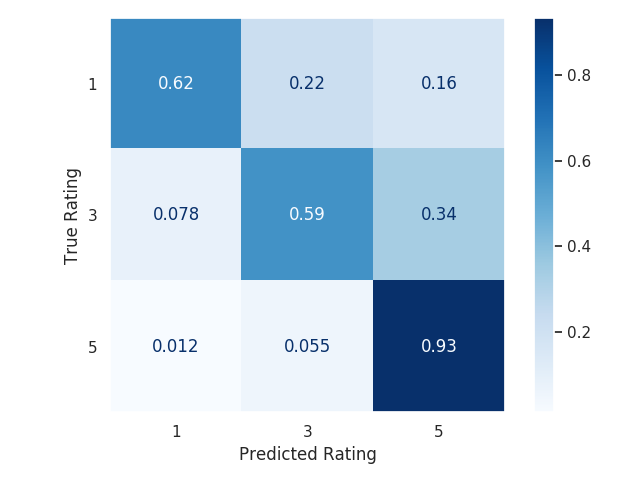
\includegraphics[width = 0.3\textwidth]{fig-linear-cm.png}
	\caption{Linear-SVM Confusion Matrix}
	\label{fig:linear-cm}
\end{figure}

\begin{figure}
	\centering
	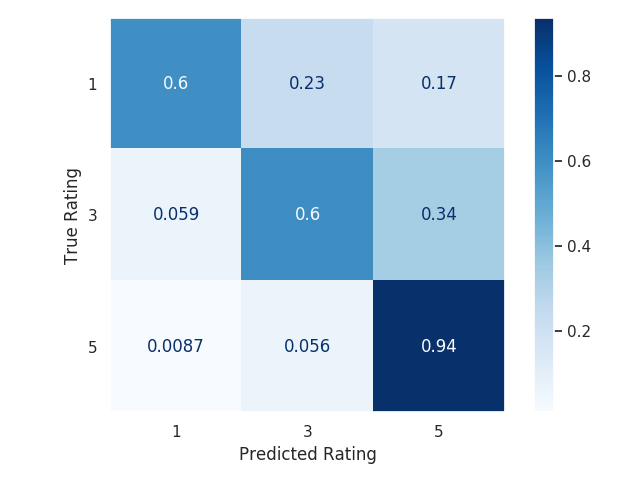
\includegraphics[width = 0.3\textwidth]{fig-rbf-cm.png}
	\caption{RBF-SVM Confusion Matrix}
	\label{fig:rbf-cm}
\end{figure}

\begin{figure}
	\centering
	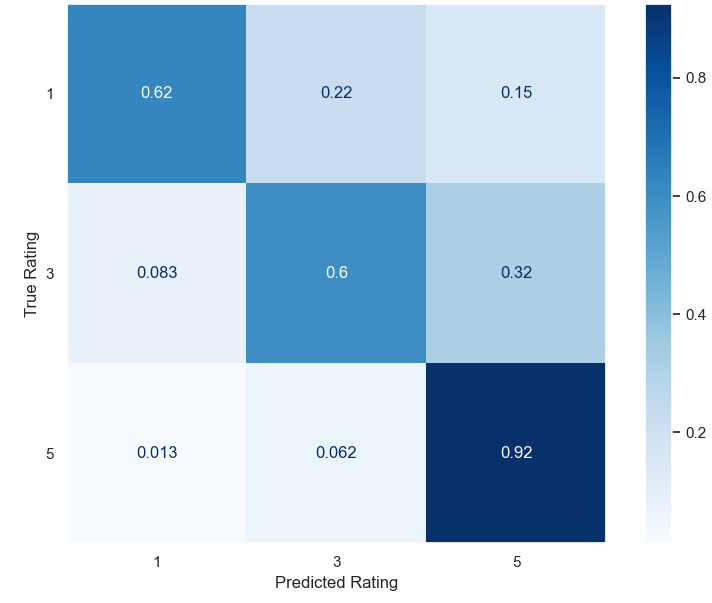
\includegraphics[width = 0.25\textwidth]{fig-lr-cm.png}
	\caption{Logistic Regression Confusion Matrix}
	\label{fig:lr-cm}
\end{figure}


\drafting{We evaluated our stacked models with the computed PVEs for a 5-fold stratified cross validation split, using the best hyperparameters for each respective base classifier, and untuned parameters for the meta-classifier (which was MLR in each case). When the base classifiers had different optimal dimensions for PVE, we selected the dimension optimal to the classifier with better sole performance. Stacking models took a long time to train and so not all dimensions could be investigated. Stacked RBF-SVM and Linear-SVM had a higher accuracy and F1-score than all other stacked models, including all 4 models stacked together. The results for this model can be seen in \ref{fig:stack-cm}}
\begin{figure}
	\centering
	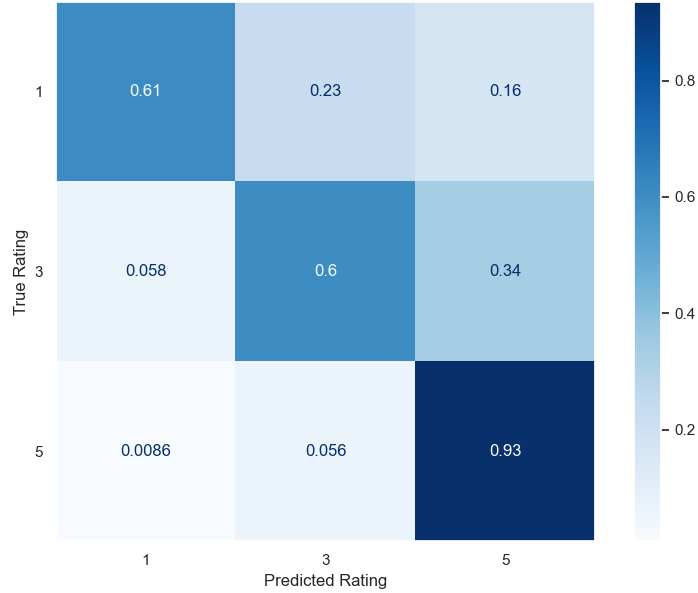
\includegraphics[width = 0.22\textwidth]{fig-stack-cm.png}
	\caption{Stacking Confusion Matrix}
	\label{fig:stack-cm}
\end{figure}

\section{Analysis}
All models achieved better accuracy than the Zero-R baseline model, which has an accuracy of $69 \%$, which shows that the models were to some degree using features to effectively make predictions. All models, including the stacking models, did not exceed an F-Score of 0.83 on unseen data. Since stacking does not improve model performance significantly, and model performance is very similar, this suggests that all models are drawing roughly the same decision boundary between the classes. This means the stacking model cannot exploit the strengths and minimise the weaknesses of the differences in the models, leading to approximately the same performance as its component models. 

Another possible reason that all models had similar performance is that this reflects the inherent difficultly of the classification task (with the selected features). It is likely that it is not possible to predict the rating enirely from the review text. Even for a human reader, the rating provides context by which to judge the sentiment of the review. For example the same review text may be interpreted as a genuine complement alongside a 5 star rating, but as sarcastic alongside a 1 star rating.

All models perform best paragraph vector encodings of around the same dimension. This suggests that this is the best dimension of paragraph vector encoding for this training corpus for representing the information in the text relevant to the rating.

Despite having the best performance of the SVM-based classifiers on unseen data, it appears that the RBF-SVM tends to overfit the training data. In Figure \ref{fig:learning-curve} we can see that the performance of RBF-SVM on the training set is significantly higher than on the test data. This is in contrast to the other classifiers, which have very similar performance on the training and testing data. This suggests RBF-SVM is learning a decision boundary which is tailored to the training data, and so, despite performing marginally worse, Linear-SVM has better generalised from the training data. This is consistent with the assumption that the data should be linearly separable discussed in Section \ref{subsec:method-svm}.

As we can see in Figures \ref{fig:binary-cm}, \ref{fig:linear-cm}, \ref{fig:rbf-cm}, \ref{fig:lr-cm} and \ref{fig:stack-cm} the main difference in performance between the models comes from their ability to distinguish the negative and neural sentiment classes. All models were, to varying degrees, biased towards predicting the text to be more positive than it was, with the upper triangle of the confusion matrix containing the most incorrect predictions. One reason for this is that the data contains mostly positive and neutral examples. If the prior probability of a class is higher, it makes sense that a classifier would predict it more frequently and thus be more often incorrect when guessing this class. Another factor in this may be is that the distinction between negative and neutral, and neutral and positive sentiment language is not very clear. This, combined with the differences in prior probability, would lead to the observed tendency of models to frequently predict one class more positive.

The Binary-SVM model (F-score of 0.758) performed worse than the Linear-SVM model (F-score of 0.821) which is consistent with results in the literature \cite{koppel_importance_2006}. This means that the assumptions about the text data discussed in Section \ref{subsec:method-svm} which would lead to good performance of the Binary-SVM model are too strong. It is likely that the language used in positive and negative reviews is not completely opposite, so paragraph vector encodings of these reviews do not lie along a line.

One major improvement we could make would be to attempt to simplify texts linguistically prior to producing the paragraph vector encodings. In the simplest case this could involve using an automated spell checker on the reviews, and in more complex cases undoing negatives (``not bad'' $\mapsto$ ``good'') and identifying common phrases or idioms. Given enough examples, the paragraph vector encoding should be able to account for this without preprocessing, since words and phrases with similar meanings should be close in the feature space. However it is likely that there are not enough examples of misspellings and unusual phrasings in the training set to do this effectively in all cases.

\drafting{more improvements?}


\section{Conclusion}
\drafting{Summarise main points and (possibly) future work.}

%put any citations here which must be included in the bibliography but won't necessarily be referenced

%citations for the dataset
\nocite{mukherjee_what_2013}
\nocite{rayana_collective_2015}

%citations for software libraries
\nocite{sklearn_pedregosa_scikit-learn_2011}
\nocite{gensim_rehurek_software_2010}
\bibliographystyle{acl}
\bibliography{report}

\end{document}
